
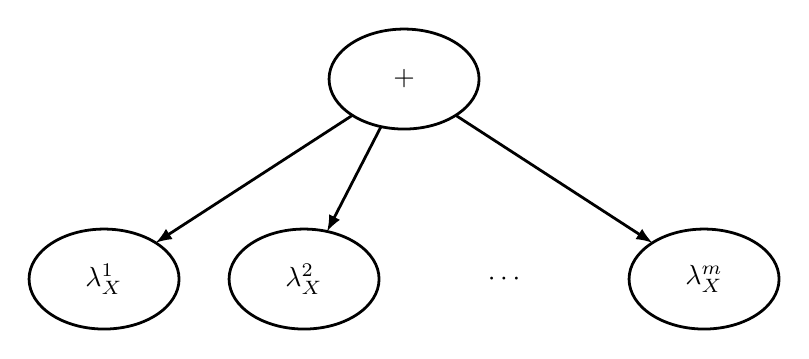
\begin{tikzpicture}[>=latex,line join=bevel,]
  \pgfsetlinewidth{1bp}
%%
\pgfsetcolor{black}
  % Edge: s -> l1
  \draw [->] (116.19bp,76.807bp) .. controls (98.998bp,65.665bp) and (73.382bp,49.062bp)  .. (45.597bp,31.053bp);
  % Edge: s -> lm
  \draw [->] (153.81bp,76.807bp) .. controls (171.0bp,65.665bp) and (196.62bp,49.062bp)  .. (224.4bp,31.053bp);
  % Edge: s -> l2
  \draw [->] (126.65bp,72.765bp) .. controls (122.29bp,64.283bp) and (116.85bp,53.714bp)  .. (107.3bp,35.147bp);
  % Node: s
\begin{scope}
  \definecolor{strokecol}{rgb}{0.0,0.0,0.0};
  \pgfsetstrokecolor{strokecol}
  \draw (135.0bp,90.0bp) ellipse (27.0bp and 18.0bp);
  \draw (135.0bp,90.0bp) node {$+$};
\end{scope}
  % Node: lm
\begin{scope}
  \definecolor{strokecol}{rgb}{0.0,0.0,0.0};
  \pgfsetstrokecolor{strokecol}
  \draw (243.0bp,18.0bp) ellipse (27.0bp and 18.0bp);
  \draw (243.0bp,18.0bp) node {$\lambda_X^m$};
\end{scope}
  % Node: l2
\begin{scope}
  \definecolor{strokecol}{rgb}{0.0,0.0,0.0};
  \pgfsetstrokecolor{strokecol}
  \draw (99.0bp,18.0bp) ellipse (27.0bp and 18.0bp);
  \draw (99.0bp,18.0bp) node {$\lambda_X^2$};
\end{scope}
  % Node: cdots
\begin{scope}
  \definecolor{strokecol}{rgb}{0.0,0.0,0.0};
  \pgfsetstrokecolor{strokecol}
  \draw (171.0bp,18.0bp) node {$\cdots$};
\end{scope}
  % Node: l1
\begin{scope}
  \definecolor{strokecol}{rgb}{0.0,0.0,0.0};
  \pgfsetstrokecolor{strokecol}
  \draw (27.0bp,18.0bp) ellipse (27.0bp and 18.0bp);
  \draw (27.0bp,18.0bp) node {$\lambda_X^1$};
\end{scope}
%
\end{tikzpicture}
